\chapter{Conceptualisation and Modelling}
\label{chp2:concept_model}


\section{System Concepts}
%WHAT you are going to present in this chapter/section
%WHY you are presenting it, and
%HOW you are going to present it
The report contains many variable names and use of terminology for concepts that is used throughout the report. These variables and terminologies are defined here.\\

The double pendulum is a under-actuated system which is defined as a system where the input to the system cannot command one of the state variables to in instantaneous change in position.\\

The robotic gymnast is describe as a double pendulum consisting out of an actuated- and non-actuated pendulum as seen in Figure \ref{fig:doublePen}. The position of the non-actuated pendulum is described by the angle $\theta$ whereas the actuated pendulum is described by $\phi$ relative to $\theta$.


underactuation, equilibrium position, unstable stable



\section{Mathematical Model}
\label{sec:math_model}
%WHAT you are going to present in this chapter/section
%WHY you are presenting it, and
%HOW you are going to present it
\begin{figure}[h]
	\centering
	
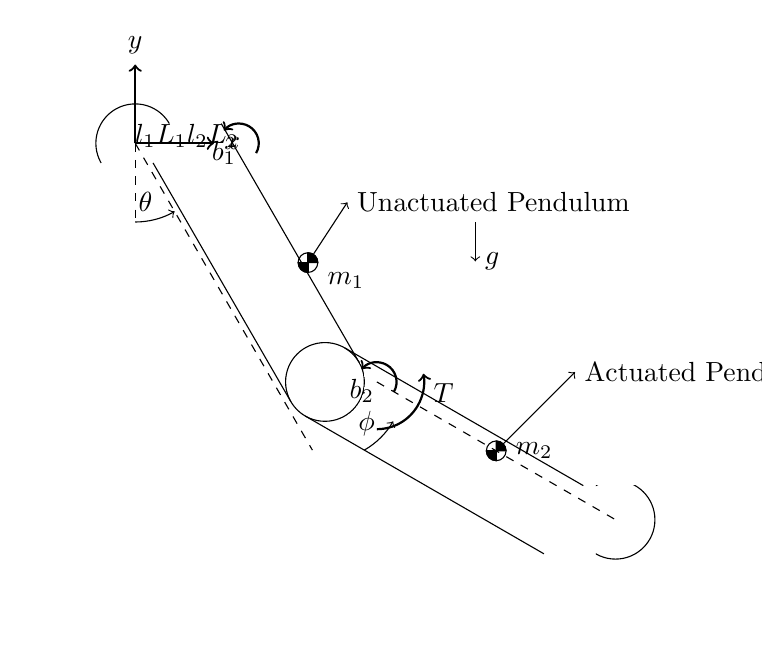
\begin{tikzpicture}[scale=0.5]

\begin{scope}
\clip [rotate=30] (-2,0) rectangle (2,2);
\draw (0,0) circle [radius=1cm];
\end{scope}

\coordinate (O) at (0,0) ;
% Second cirle middle point
\coordinate (A) at (3.5,-6.06217); 
\coordinate (B) at (3.5+6.06217,-6.06217-3.5); 
	% Lenght of pendulums are 7cm

	% Axis for underactuated Pendulum
	\draw[->,thick] (0,0) -- (2,0) node[anchor=west] {$x$};
	\draw[->,thick] (0,0) -- (0,2) node[anchor=south] {$y$};
	\draw[dashed] (0,0) -- (0,-2);
	
	%%%%%%%%%%%%%%%%%%%%%%%%%%%%%%%%%%%%%%%%%%%%%%%%%%%%%%%%%%%%%%%%%%%%%%%%%%%%%%
							%% Theta %%
	\begin{scope}
		\draw[->] (0,-2) arc (270:300:2);
		\draw (280:1.5) node {$\theta$};
	\end{scope}
	%%%%%%%%%%%%%%%%%%%%%%%%%%%%%%%%%%%%%%%%%%%%%%%%%%%%%%%%%%%%%%%%%%%%%%%%%%%%%%
	
	%%%%%%%%%%%%%%%%%%%%%%%%%%%%%%%%%%%%%%%%%%%%%%%%%%%%%%%%%%%%%%%%%%%%%%%%%%%%%%
				%% Middle line for underactuated pendulum %%
	\draw[dashed] (0,0) -- (4.5,-7.79422);
	%%%%%%%%%%%%%%%%%%%%%%%%%%%%%%%%%%%%%%%%%%%%%%%%%%%%%%%%%%%%%%%%%%%%%%%%%%%%%%
	
		
	%%%%%%%%%%%%%%%%%%%%%%%%%%%%%%%%%%%%%%%%%%%%%%%%%%%%%%%%%%%%%%%%%%%%%%%%%%%%%%
					%% Dimensions of underactuated Pendulum %%
	\dimline[line style = {line width=0.7},extension start length=-0.25, extension end length=-0.4]{(-1.732,-1)}{(-1.732+1.75,-1-3.031)}{$l_{1}$}
	
	\dimline[line style = {line width=0.7},extension start length=-0.25, extension end length=-0.25]{(-2.598,-1.5)}{(-2.598+3.5,-1.5-6.06217)}{$L_{1}$}
	
	%%%%%%%%%%%%%%%%%%%%%%%%%%%%%%%%%%%%%%%%%%%%%%%%%%%%%%%%%%%%%%%%%%%%%%%%%%%%%%

	%Long lines for underactuated pendulum
	\draw (0.8660,0.5) -- (0.866+3.5,0.5-6.06217);
	\draw (-0.8660,-0.5) -- (-0.866+3.5,-0.5-6.06217);	
	
	
	
	%%%%%%%%%%%%%%%%%%%%%%%%%%%%%%%%%%%%%%%%%%%%%%%%%%%%%%%%%%%%%%%%%%%%%%%%%%%%%%
					%% Middle circle for both pendulums %%
	\begin{scope}
		%\clip [rotate=00] (0.866+3.5,0.5-6.06217+2) rectangle (-0.866+3.5-2,-0.5-6.06217);
	\clip (A) circle [radius=1.02];
	\draw (A) circle [radius=1cm];
	\end{scope}
	
	%\draw [rotate=00] (0.866+3.5,0.5-6.06217+2) rectangle (-0.866+3.5-2,-0.5-6.06217);
	
	%%%%%%%%%%%%%%%%%%%%%%%%%%%%%%%%%%%%%%%%%%%%%%%%%%%%%%%%%%%%%%%%%%%%%%%%%%%%%%
	% Axis for lower Pendulum
	%\draw[->,thick] (3.5,-6.06217) -- (6.5,-6.06217) node[anchor=west] {$x_{2}$};
	%\draw[->,thick] (3.5,-6.06217) -- (3.5,-3.06217) node[anchor=south] {$y_{2}$};
	%\draw[dashed] (3.5,-6.06217) -- (3.5,-8.56217);
	
	% Long lines for actuated pendulum
	\draw (3.5+0.5,-6.06217+0.86602) -- (3.5+0.5+6.06217,-6.06217+0.86602-3.5);
	\draw (3.5-0.5,-6.06217-0.86602) -- (3.5-0.5+6.06217,-6.06217-0.86602-3.5);
	
	%%%%%%%%%%%%%%%%%%%%%%%%%%%%%%%%%%%%%%%%%%%%%%%%%%%%%%%%%%%%%%%%%%%%%%%%%%%%%%
							%%  Phi %%
	\begin{scope}
	\draw[->] (4.5,-7.79422) arc (300:330:2);
	
	
	\draw (3.5,-6.06217)+ (315:1.5) node {$\phi$};
	\end{scope}
	%%%%%%%%%%%%%%%%%%%%%%%%%%%%%%%%%%%%%%%%%%%%%%%%%%%%%%%%%%%%%%%%%%%%%%%%%%%%%%
	
	%%%%%%%%%%%%%%%%%%%%%%%%%%%%%%%%%%%%%%%%%%%%%%%%%%%%%%%%%%%%%%%%%%%%%%%%%%%%%%
						%% Dimensions of actuated Pendulum %%
	\dimline[line style = {line width=0.7},extension start length=-0.25, extension end length=-0.4]{(2.5,-7.79421)}{(5.53108,-9.54422)}{$l_{2}$}
	
	\dimline[line style = {line width=0.7},extension start length=-0.25, extension end length=-0.25]{(2,-8.66028)}{(8.06217,-12.1602)}{$L_{2}$}
	
	%%%%%%%%%%%%%%%%%%%%%%%%%%%%%%%%%%%%%%%%%%%%%%%%%%%%%%%%%%%%%%%%%%%%%%%%%%%%%%

	
	%%%%%%%%%%%%%%%%%%%%%%%%%%%%%%%%%%%%%%%%%%%%%%%%%%%%%%%%%%%%%%%%%%%%%%%%%%%%%%
							%% Circle at the bottom %%
	\begin{scope}
	\clip [rotate=00] (3.5+0.5+6.06217+2,-6.06217+0.86602-3.5) rectangle ((3.5-0.5+6.06217,-6.06217-0.86602-3.5-2);
	\draw (B) circle [radius=1cm];
	\end{scope}
	%%%%%%%%%%%%%%%%%%%%%%%%%%%%%%%%%%%%%%%%%%%%%%%%%%%%%%%%%%%%%%%%%%%%%%%%%%%%%%

	
	%%%%%%%%%%%%%%%%%%%%%%%%%%%%%%%%%%%%%%%%%%%%%%%%%%%%%%%%%%%%%%%%%%%%%%%%%%%%%%
					%% Middle line for actuated pendulum %%
	\draw[dashed] (3.5,-6.06217)--(3.5+6.06217,-6.06217-3.5);
	%%%%%%%%%%%%%%%%%%%%%%%%%%%%%%%%%%%%%%%%%%%%%%%%%%%%%%%%%%%%%%%%%%%%%%%%%%%%%%
		
	%%%%%%%%%%%%%%%%%%%%%%%%%%%%%%%%%%%%%%%%%%%%%%%%%%%%%%%%%%%%%%%%%%%%%%%%%%%%%%
				%% Centroid symbol for underactuade pendulum %%
	\draw (1.75,-3.0310) circle [radius=0.25cm];
	\draw (1.75-0.25,-3.0310) -- (1.75+0.25,-3.0310)  node[below right]{$m_{1}$};`
	\draw (1.75,-3.0310+0.25) -- (1.75,-3.0310-0.25);
	\filldraw[fill=black,draw=black] (1.75,-3.0310) -- (1.75+0.25,-3.0310)
		arc[start angle = 0, end angle = 90, radius = 0.25] -- cycle;
		
	\filldraw[fill=black,draw=black] (1.75,-3.0310) -- (1.75-0.25,-3.0310)
	arc[start angle = 180, end angle = 270, radius = 0.25] -- cycle ;
	%%%%%%%%%%%%%%%%%%%%%%%%%%%%%%%%%%%%%%%%%%%%%%%%%%%%%%%%%%%%%%%%%%%%%%%%%%%%%%
	
	%%%%%%%%%%%%%%%%%%%%%%%%%%%%%%%%%%%%%%%%%%%%%%%%%%%%%%%%%%%%%%%%%%%%%%%%%%%%%%
				%% Centroid symbol for actuaded pendulum %%
	\draw (6.53108,-7.81217) circle [radius=0.25cm];
	\draw (6.53108-0.25,-7.81217) -- (6.53108+0.25,-7.81217)  node[right]{$m_{2}$};
	\draw (6.53108,-7.81217+0.25) -- (6.53108,-7.81217-0.25);
	\filldraw[fill=black,draw=black] (6.53108,-7.81217) -- (6.53108+0.25,-7.81217)
	arc[start angle = 0, end angle = 90, radius = 0.25] -- cycle;
	
	\filldraw[fill=black,draw=black] (6.53108,-7.81217) -- (6.53108-0.25,-7.81217)
	arc[start angle = 180, end angle = 270, radius = 0.25] -- cycle ;
	%%%%%%%%%%%%%%%%%%%%%%%%%%%%%%%%%%%%%%%%%%%%%%%%%%%%%%%%%%%%%%%%%%%%%%%%%%%%%%
	
	% Torque Input
	%\draw[->,thick] (3.5,-7.5) to [bend right] (5.25,-4.76314) node[right]{$T$}; 
	\draw[->,thick] (A) +(0,-1.2) arc (270:370:1.2) node[below right] {$T$};
	
	
	% Damping in bearings
	\draw[->,thick] (0.433,-0.25) arc (330:500:0.5) node[below] {$b_{1}$};
	
	% Damping between motor rotor and stator 
	\draw[->,thick] (A)+(0.433,-0.25) arc (330:500:0.5) node[below] {$b_{2}$};
	
	% Direction of gravity
	\draw[->] (6,-2)--(6,-3) node[right]{$g$};
	
	% Labels for pendulums
	\draw[->] (1.75,-3.0310)--(2.75,-1.5) node[right]{Unactuated Pendulum};
	\draw[->] (6.53108,-7.81217)--(8.53108,-5.81217) node[right]{Actuated Pendulum};
	
	
\end{tikzpicture}
	\caption{Free Body Diagram of the Double Pendulum}
	\label{fig:doublePen}
\end{figure}

The approach taken to derive the mathematical model of the robotic gymnast will be discussed in this section. It is presented to allow the reader to understand parameters mentioned in the report. The swing-up of the robotic gymnast consist of non-linear behaviour and is require to fully derive the dynamics of the system. The strenuous mathematical steps are removed from the reader, which is provided in Appendix \ref{sec:math_model}, and a summary of the motivation and paradigm approach to the derivation is provided here.\\

The robotic gymnast is modelled as two pendulums connected together with a hinge, where each pendulum is modeled as having their mass distributed arbitrary along their axis. There is a torque actuating the lower pendulum seen in Figure \ref{fig:doublePen} and friction is modelled as proportional to the angular velocity of the pendulums. The friction that develops at the hinge is proportional to the relative motion of the actuated pendulum and non-actuated pendulum. The angle, $\phi$ was purposefully chosen relative to $\theta$ to ease the identification of this friction. Figure \ref{fig:doublePen} displays the free body diagram of the robotic gymnast.\\

Deriving the equation of motion of the robotic gymnast can be approached using different methods. The method chosen in the report is by using the Euler-Lagrange equation. The Euler-Lagrange equation shown in (\ref{eq:euler_lagrange_expanded}) derives the dynamics of the system by analysing the energy of the system.  This approach was chosen due to the energy of the system being easily defined as the potential energy $T$ of the 2 pendulums, and the kinetic energy $V$ of the pendulums.
 
\begin{equation} \label{eq:euler_lagrange_expanded}
\frac{d}{dt}\frac{\partial\mathcal{L}}{\partial\vec{\dot{q}}}-\frac{\partial\mathcal{L}}{\partial q} = 0
\end{equation}

\begin{equation} \label{eq:euler_lagrane}
\mathcal{L}=T-V
\end{equation}

Using the Euler-Lagrange equation leads to the condense equations ofm otions shown in (\ref{eq:condense1}) and (\ref{eq:condense2}),
\begin{equation} \label{eq:condense1}
d_{11}\ddot{\theta}+d_{12}\ddot{\phi} + h_{1} + \psi_{1} = 0
\end{equation}
\begin{equation} \label{eq:condense2}
d_{21}\ddot{\theta} + d_{22}\ddot{\phi} + h_{2} + \psi_{2} = \tau
\end{equation}
where the coefficients are defined as
\begin{equation} \label{eq:d11}
d_{11} = I_{a} + I_{b} + m_{2}(L_{1}^2 + l_{2}^2+2L_{1}l_{2}\cos(\phi))
\end{equation}
\begin{equation} \label{eq:d12}
d_{12} = I_{b} +m_{2}(l_{2}^2 L_{1}l_{2}\cos(\phi))
\end{equation}
\begin{equation} \label{eq:h1}
h_{1} = -m_{2}L_{1}l_{2}\sin(\phi)\dot{\phi^2}-2m_{2}L_{1}l_{2}\sin(\phi)\dot{\phi}\dot{\theta}
\end{equation}
\begin{equation} \label{eq:psi1}
\psi_{1} = (m_{2}l_{1}+m_{2}L_{1})g\cos(\theta) + m_{2}l_{2}g\cos(\theta+\phi)
\end{equation}
\begin{equation} \label{eq:d21}
d_{21}= I_{b}+m_{2}(l_{2}^2+L_{1}l_{2}\cos(\phi))
\end{equation}
\begin{equation} \label{eq:d22}
d_{22}= I_{b}+ m_{2}l_{2}^2
\end{equation}
\begin{equation} \label{eq:h2}
h_{2}= m_{2}L_{1}l_{2}\sin(\phi)\dot{\theta^2}
\end{equation}
\begin{equation} \label{eq:psi2}
\psi_{2}= m_{2}l_{2}g\cos(\theta+\phi)
\end{equation}

\section{Simulation Model}
	%WHAT you are going to present in this chapter/section
%WHY you are presenting it, and
%HOW you are going to present it
The mathematical model derived in the previous section is required to be implemented on a simulation program. Simulating the model allows the designer to understand how system parameters influence the dynamics of the system and the verification of controllers implemented. It will be presented by discussing how the simulation is a true representation of the system, how design specifications were determined and the influence of these parameters.\\

Simulation of the robotic gymnast was done using MATLAB Simulink. The differential equations shown in equation (\ref{eq:condense1}) and (\ref{eq:condense2}) were implemented using the MATLAB function box. It was required to write these equation where $\ddot{\phi}$ and $\ddot{\theta}$ is the subject in each of the \textit{MATLAB Function} box to allow MATLAB to simulate the model.\\

Other non-linearities introduced by sensors and components were added such as saturation of the motor, gearbox backlash and quantisation of sensory data. These non-linearities were implemented to allow the simulation to be an acceptable representation of the physical system. The Simulink Model is shown in Figure \ref{fig:sim_nonlinearfeedback}.

\begin{figure}[h]
	\centering
	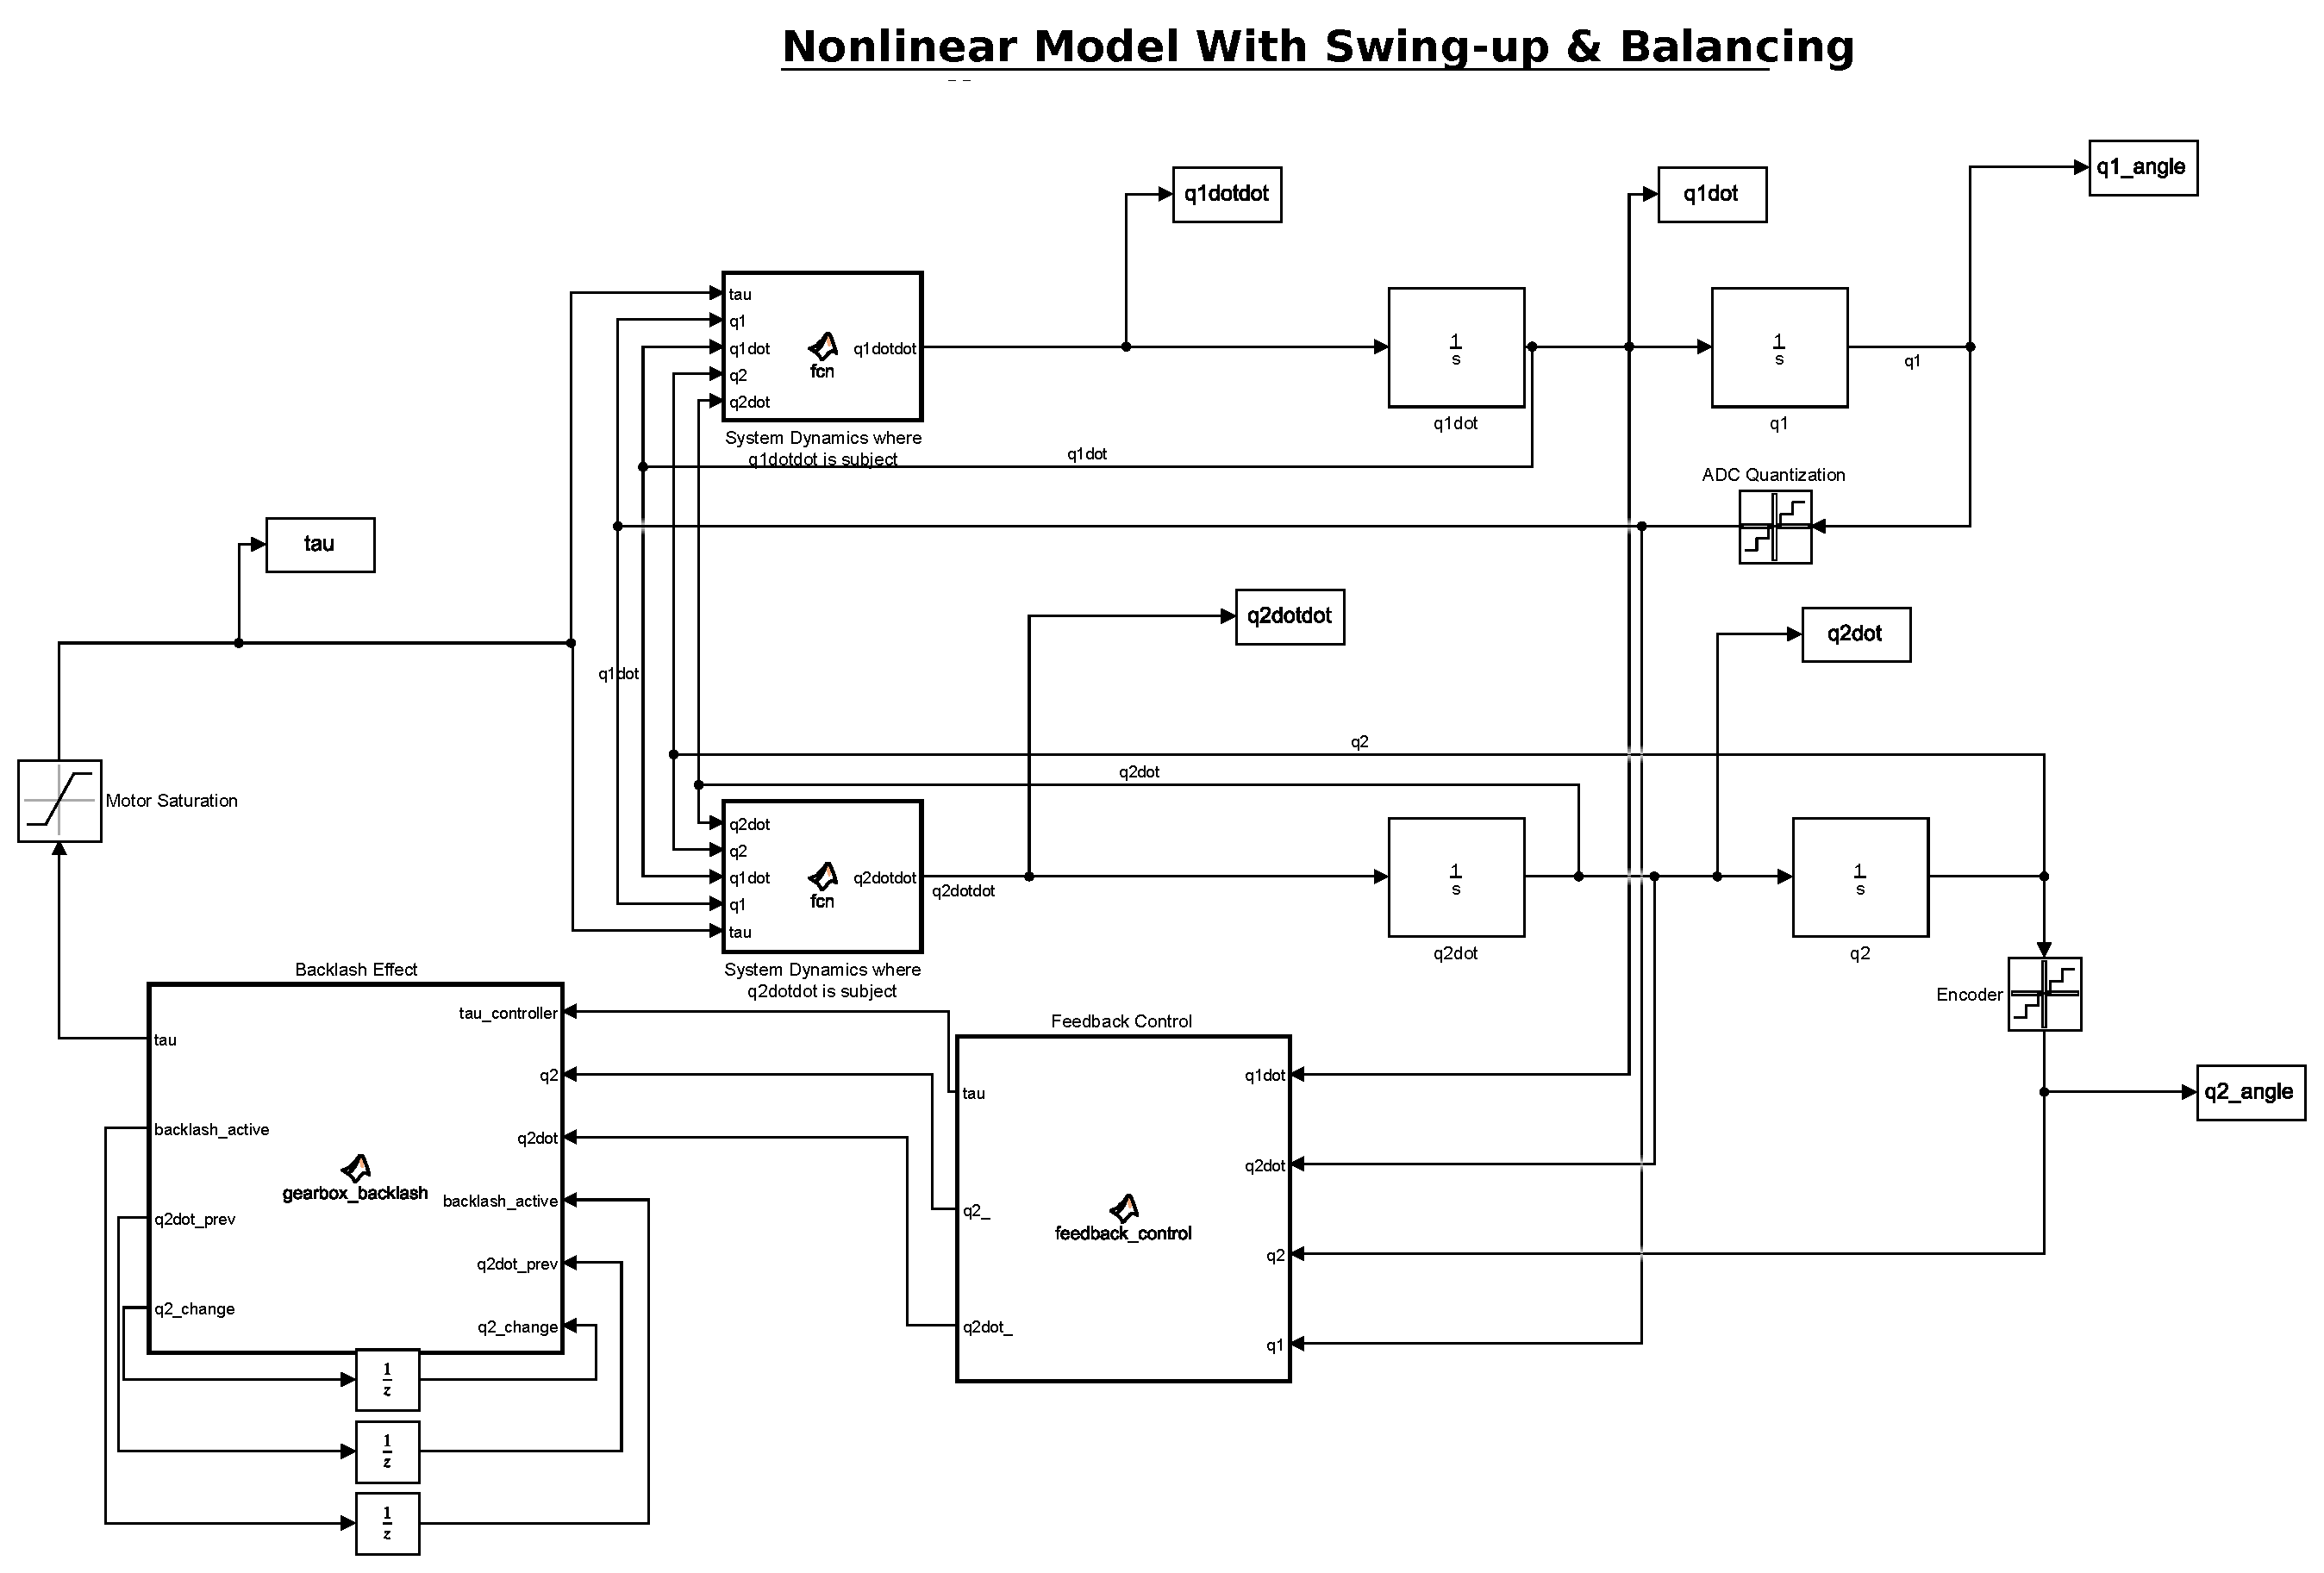
\includegraphics[scale=0.3]{./figs/simulink/simulink_model.eps}
	\caption{MATLAB Simulink Model}
	\label{fig:sim_nonlinearfeedback}
\end{figure}

\section{System Identification}
%WHAT you are going to present in this chapter/section
%WHY you are presenting it, and
%HOW you are going to present it?

The system identification tests are done to determine the characteristics that describe the behavior of the system. These characteristics include the damping ratio's and natural frequencies of the system around the unstable equilibrium position. The system are described by 2 independent parameters, $\theta$ and $\phi$ which defines the position of the non-actuated and actuated pendulums.

The project started off with a previous physical model which provided realistic system parameters to allow the simulation to be a acceptable representation of reality. From using these previous system parameters the simulation provided a set of specification for the new design. The newly design model parameters are used throughout the report and the system identification is provided here to proof the simulation is a acceptable representation of the physical model. The physical model parameters is shown in Table \ref{table:system_param}.

		\begin{table}[]
	\centering
	\begin{tabular}{|c|c|}
		\hline
		System Parameter & Value \\
		\hline
		\hline
		$L_{1}$ & \SI{0.235}{m} \\
		\hline
		$L_{2}$ & \SI{0.245}{m} \\ 
		\hline
		$I_{A}$ & \SI{0.0265}{kg\cdot m^2}\\
		\hline
		$I_{B}$ & \SI{0.0221}{kg\cdot m^2}\\
		\hline
		$m_{1}$ & \SI{0.5763}{kg}\\
		\hline
		$m_{2}$ & \SI{0.4928}{kg} \\
		\hline
		$l_{1}$ & \SI{0.235}{m}\\
		\hline
		$l_{2}$ & \SI{0.245}{m}\\
		\hline
	\end{tabular}
	\caption{System Parameters}
	\label{table:system_param}
\end{table}


Since the system is described by 2 independent parameters the system is thus a 2 degree of freedom (2DOF) system and is expected to contain 2 natural frequencies each accompanied by a damping coefficient.

The first natural frequency of the system is determine by inspecting the response of the system when starting at a initial condition and keeping $\phi = \SI{0}{rad}$ constant throughout the response. This was done by using a lightweight PVC pipe that has negligible effect on the weight of the system. The actuated pendulum and non-actuated pendulum are constrained to this pipe to ensure the 2 pendulums stay in-line with each other and thus ensuring $\phi = \SI{0}{rad}$. The response of the system is shown in Figure \ref{fig:q1_response} starting at a initial condition of roughly $\theta = \frac{\pi}{2}$. The accuracy of the initial conditions is of little importance, but the initial condition must allow the response to contain a few oscillation to accurately determine the parameters of interest.\\

\begin{figure}[h]
	\centering
	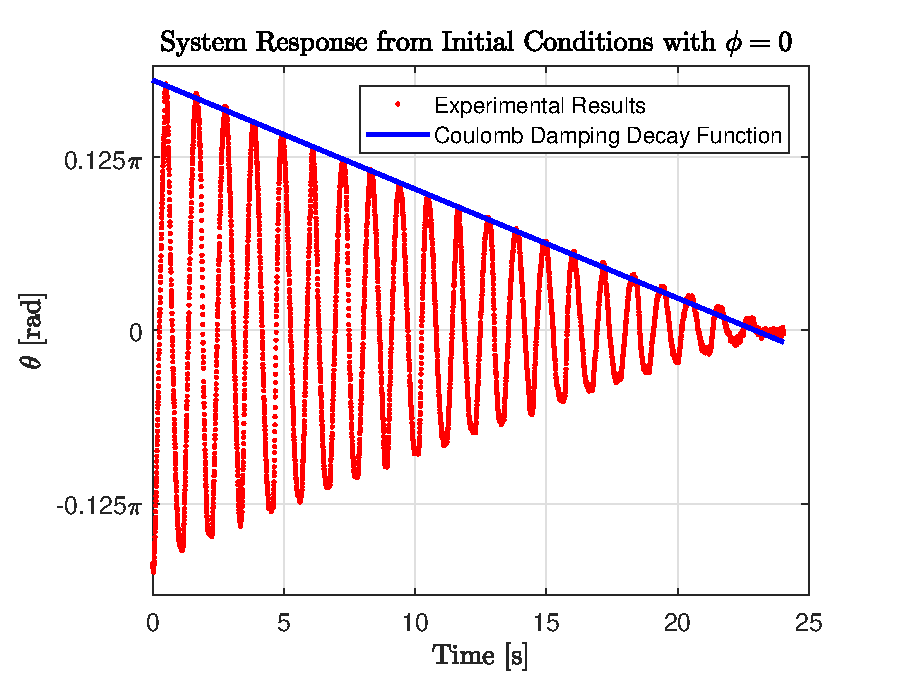
\includegraphics[scale=1]{./figs/q1_initial_response.eps}
	\caption{Initial Condition System Response while $ \phi = \SI{0}{rad} $ }
	\label{fig:q1_response}
\end{figure}


The second natural frequency is determined by analysing the response of the system when $\phi$ starting at a initial condition and keeping $\theta = \SI{0}{rad}$ throughout the response. This was accomplished by constraining the non-actuated pendulum using hard stops. Figure \ref{fig:q2_response} shows the measured response of the system when $\phi$ starts at a initial condition and keeping $\theta$ constant.

\begin{figure}[h]
	\centering
	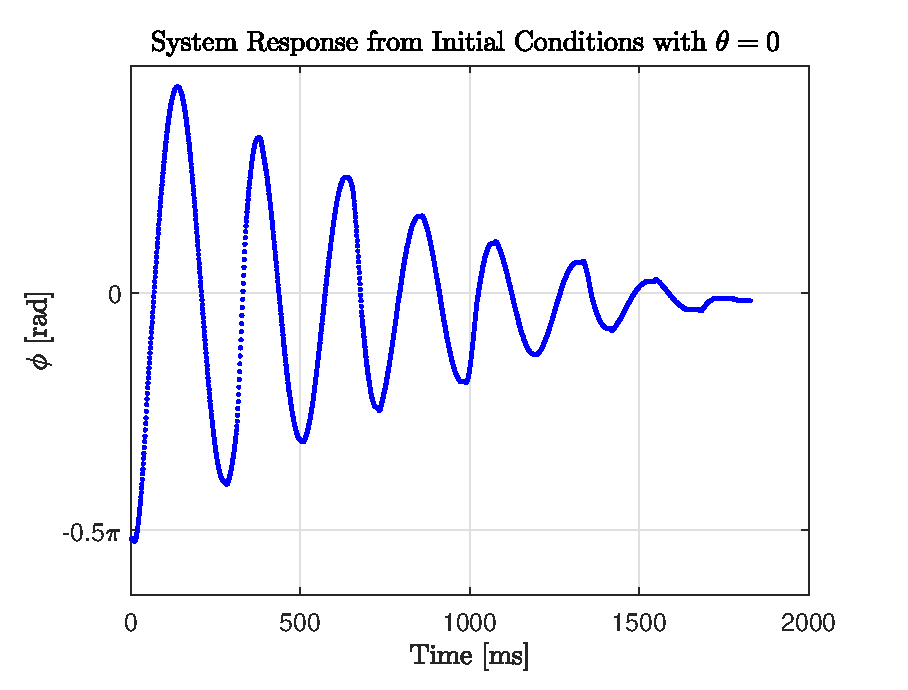
\includegraphics[scale=1]{./figs/q2_initial_response.eps}
	\caption{Initial Condition System Response while $ \theta = \SI{0}{rad} $ }
	\label{fig:q2_response}
\end{figure}

The natural frequencies of the system is identified by inspecting the frequency content of the time-domain responses. The frequency content of the initial condition responses of both experiments are shown in Figure \ref{fig:fft_system_response}, by applying the Fast Fourier Transform (FFT) algorithm to the time-domain signals. The FFT indicates the natural frequencies by the predominant peaks across the frequency spectrum which are tabulated in Table \ref{table:system_characteristic}.\\

\begin{figure}[h]
	\centering
	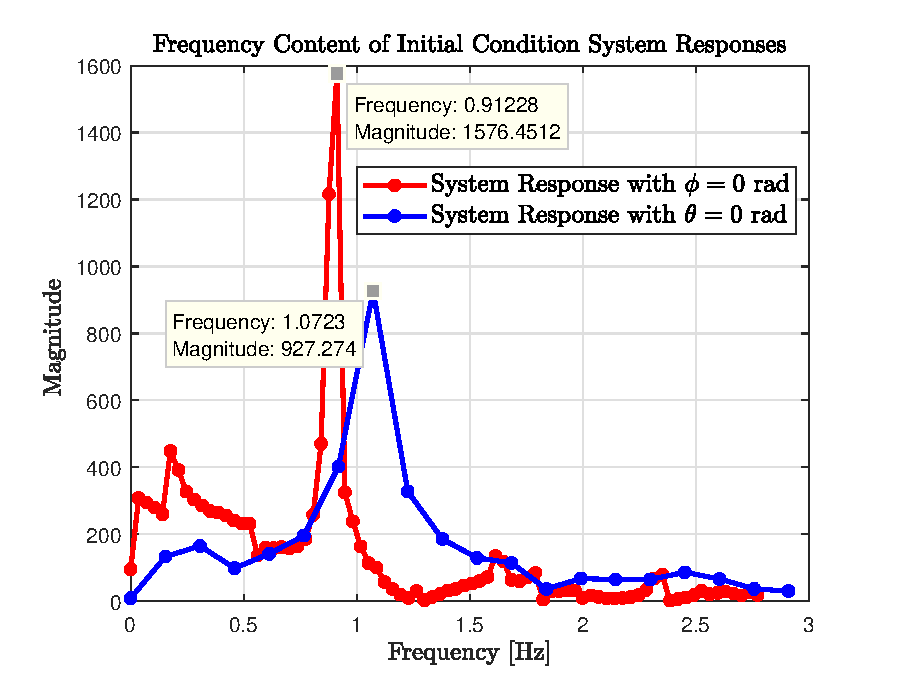
\includegraphics[scale=1]{./figs/FFT_system.eps}
	\caption{Frequency Content of Time-Domain Initial Condition Responses}
	\label{fig:fft_system_response}
\end{figure}

The responses shown in Figure \ref{fig:q1_response} and \ref{fig:q2_response} are decaying with time and this decaying behaviour can be modeled by the following equation: $$\tau(t) = -\zeta \omega_{n} t$$ Where $\omega_{n}$ is the natural frequency of the system and $\zeta$ the damping ratio of the system. The natural frequencies of the system has already been determined and thus linear regression can be used to determine the best $\zeta$ that will fit the measured data. The decaying functions are shown in Figure \ref{fig:q1_response} and \ref{fig:q2_response} with the best fit $\zeta$ values shown in Table \ref{table:system_characteristic}. It is visible from the responses that the damping ratio changes when the response are nears steady state. This change of damping ratio is neglible due to the controllers being implement are robust to changes in $\zeta$.

\begin{table}[]
	\centering
	\begin{tabular}{|c|c|c|c|}
		\hline
		System Characteristic & Mean & Standard Deviation\\
		\hline
		\hline
		$f_{1}$ & \SI{3.93}{Hz} &  \\
		\hline
		$f_{2}$ & \SI{3.62}{Hz} & 0.04029 \\ 
		\hline
		$\zeta_{1}$ & $1.6931 \cdot10^{-5}$ & $4.823\cdot 10^{-6}$
		\\
		\hline
		$\zeta_{2}$ & $5.85184 \cdot 10^{-5}$ & \\
		\hline
	\end{tabular}
	\caption{System Characteristic \& their Statistical Properties from 10 Experiments}
	\label{table:system_characteristic}
\end{table}

Figure \ref{fig:q1_response} shows the decaying function with properties that are shown in Table \ref{table:system_response_prop} and it is visible that the calculated values provides a acceptable approximation of the measured data.

\section{Model Validation}
%WHAT you are going to present in this chapter/section
%WHY you are presenting it, and
%HOW you are going to present it?
The model implemented in simulation must be able describe the physical model to an acceptable degree to allow any further developments on the simulated model. The simulated model will be validated by comparing the experimental system characteristic values to those attained in simulation.
 
\begin{table}[]
	\centering
	\begin{tabular}{|c|c|c|c|}
		\hline
		System Characteristic & Experiment & Simulated & Difference\\
		\hline
		\hline
		$w_{{n}_{1}}$ & \SI{3.93}{Hz} & & \\
		\hline
		$w_{{n}_{2}}$ & \SI{3.62}{Hz} & 0.04029 &\\ 
		\hline
	\end{tabular}
	\caption{Comparison between Experimental- and Simulated System Characteristic}
	\label{table:simulate_vs_experiment}
\end{table}
